
\section{\acl{dl}-Based \ac{ser}}

This section presents the exploration of using deep learning classifiers for audio-based emotion recognition, focusing on the use of various features for the classification task.

\subsection{\acl{dl} Features}

Initially, three different features were extracted from the raw audio signals, using the Librosa library. The numeric values of the extracted features were saved into a Pickle file, while the visual representation of the feature was saved as a Portable Network Graphic (PNG) file. The PNG file was generated using a Matplotlib figure with 100 dots per inch, without the axis and the frame. The color map used was \textit{viridis\_r}.

The 2D deep learning models employed in this study required the input data to possess consistent dimensions. To this end, the numeric data of every feature used only the first 6 seconds of every audio file, with shorter audio signals padded with trailing zeros to achieve the required length.

The first feature explored was the spectrogram. The Short-time Fourier transform (STFT) was used to calculate the spectrogram, using a windowed signal length of 2048, after padding with zeros. This resulted in matrices with a dimension of $1025x188$. The amplitude spectrogram was converted to a dB-scaled spectrogram, which was then used for the PNG file.

Another feature explored was the Mel Spectrogram. For this, the previously calculated spectrogram was mapped onto the mel scale, using 256 Mel bands. This resulted in matrices with a dimension of $256x188$. The dB-scaled Mel Spectrogram was also used for the PNG file.

The third feature explored was the \ac{mfccs} as they are commonly used for audio signal processing tasks due to their ability to capture the spectral characteristics of audio signals. 40 \ac{mfccs} were extracted from the previously calculated Mel Spectrogram, resulting in matrices with a dimension of $40x188$.

These three used features are displayed in figure \ref{fig:dl_features}.

\begin{figure}[H]
	\centering
	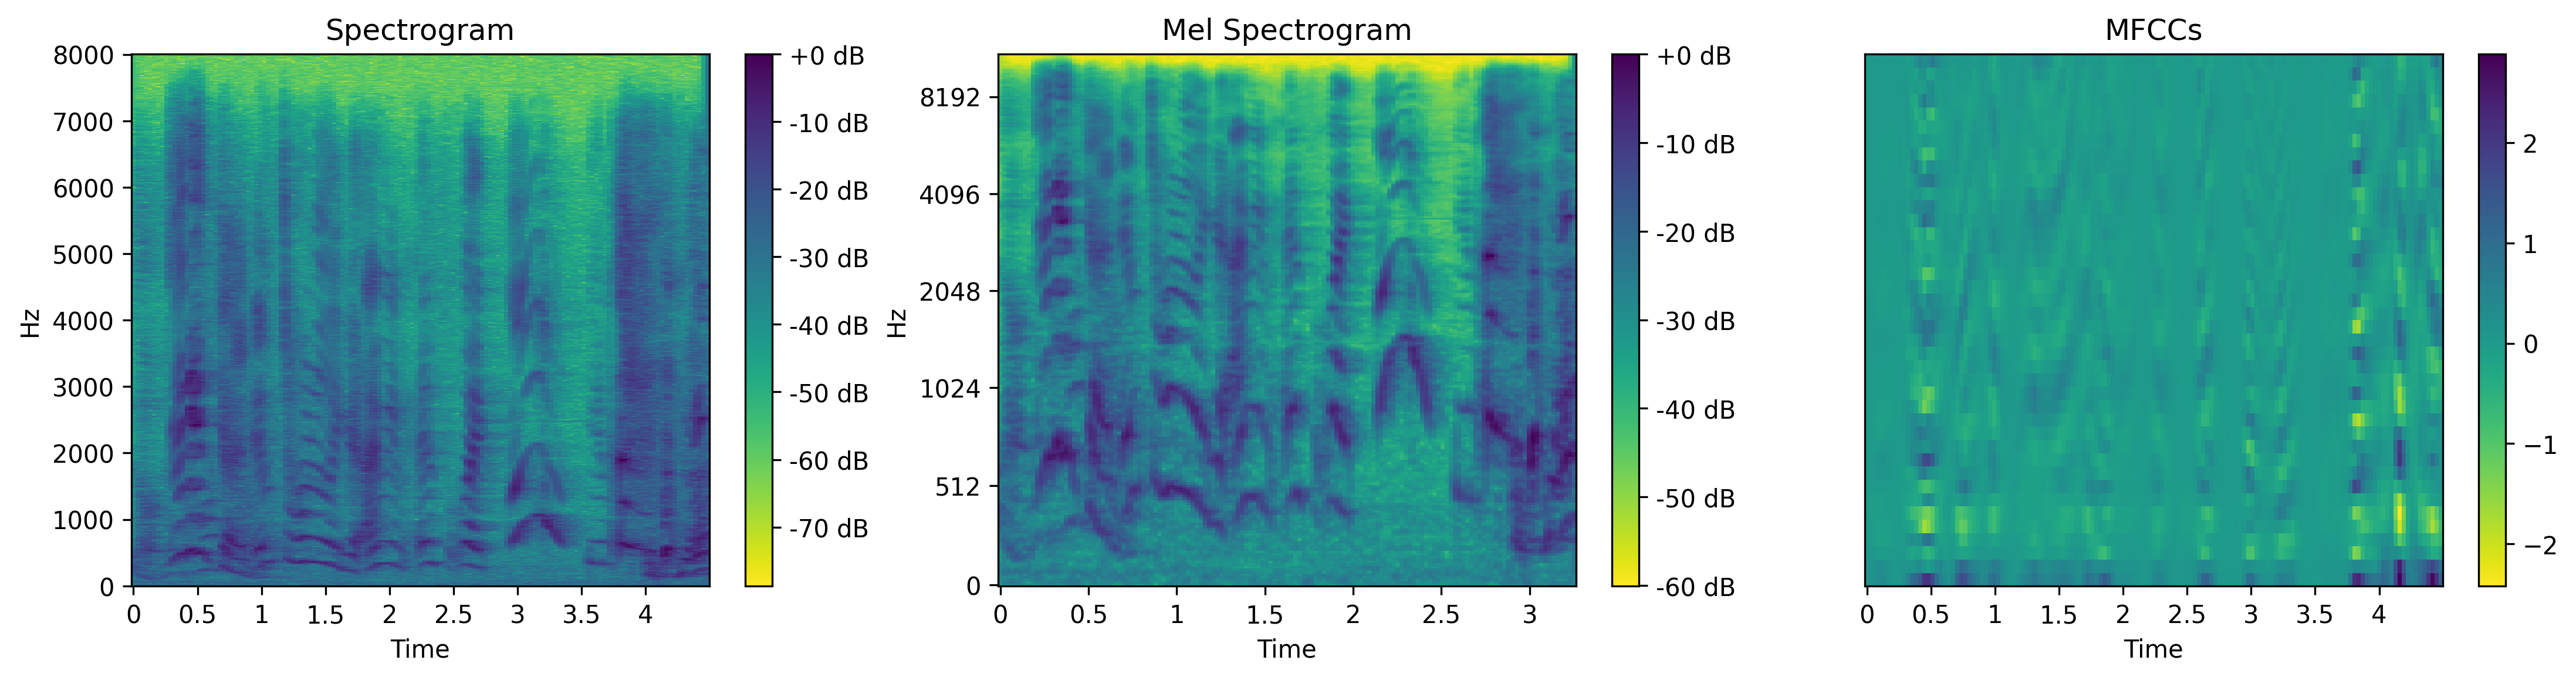
\includegraphics[width=\textwidth]{figs/4_4_deep_learning/features.png}
	\caption{Graphical representations of the features used as input for the \ac{dl} classifiers.}
	\label{fig:dl_features}
\end{figure}



\subsection{Classifiers Evaluation and Selection}

\subsubsection{Evaluation Strategy}

The classifiers were trained using a Tesla P4 GPU on the Google Colab service. In order to evaluate the performance of the classifiers, 5-fold cross-validation was performed using the stratified K-fold strategy to preserve the percentage of samples for each class. The models were trained for 80 epochs, with a batch size of 128 and a learning rate decay of 10\% every 10 epochs. The Adam optimizer was used for all models with a learning rate of 0.001.

The evaluation of the classifiers was done based on various metrics including accuracy, precision, recall, and macro F1-score. The training time was also annotated and the corresponding confusion matrices were also plotted, present in the appendix \ref{METER DPS}. These metrics were computed using the average across the 5 folds, without using class weights, to give an overall performance overview of the classifier.

\subsubsection{Numeric Data Classification}


\subsubsection{Image Classification}

In our study of deep learning-based \ac{ser} using images, we utilized transfer learning techniques with three different pre-trained models: ResNet50, VGG16, and Xception.

ResNet50, VGG16, and Xception are popular deep convolutional neural networks (CNN) that have shown outstanding performance in various computer vision tasks, including image classification. We used the pre-trained versions of them on the large-scale ImageNet dataset, which contains millions of labeled images belonging to thousands of different classes. This means their weights and biases have already been adjusted for the ImageNet dataset, and they have learned how to extract meaningful features from images, which helps improving the accuracy and generalization ability of the models, as it allows them to recognize patterns and shapes that are common across a wide range of images.

To prepare the data for these models, we loaded the images with a dimension of $224x224x3$ using the TensorFlow Keras \textit{load\_img} function from the \textit{preprocessing.image} module. The images were then converted into arrays using the \textit{img\_to\_array} function from the same module. In addition, before inputting the data into the models, we applied the respective preprocessing technique for each classifier. For example, we used the \textit{preprocess\_input} function from the Tensorflow  Keras \textit{applications.resnet50} module for the ResNet50 classifier.

In the transfer learning technique, all layers of the chosen classifier were frozen, and a new Dense layer with 64 units with \textit{relu} activation was added to the model. A Dropout layer with a 0.5 rate was then included to avoid overfitting, followed by a Dense layer with 4 units with \textit{softmax} activation to output the predicted emotion.

Through the implementation of these pre-trained models with transfer learning, we aim to harness their robust feature extraction abilities and significantly reduce the training duration required for the inherently computationally intensive 3D classification task at hand.


\subsubsection{Results and Conclusions}

Table \ref{tab:dl_models} displays the results obtained. The outcomes of the experiments illustrate the efficacy of employing transfer learning with pre-trained models for the task of \ac{ser}. While the spectrogram image feature attained the highest average accuracy when utilizing the Resnet50 model and weights, the mel spectrogram feature achieved the best overall performance across all models. Furthermore, the image of the mel spectrogram obtained the second-highest accuracy with the Resnet50 model and displayed a smaller standard deviation, indicating that it performed comparably well in all cross-validation folds.

From these results we noted the Resnet50 model with Spectrogram Images as input as the best deep learning candidate as it obtained the highest values on all metrics.

\begin{table}[H]
	\centering
	\caption{\ac{dl} Classification Models Performance on \ac{iemo}.}
	\label{tab:dl_models}
	\resizebox{\textwidth}{!}{%
		\begin{tabular}{llrrrrrr}
			\toprule
			Feature & Model & Accuracy & Macro F1 & Precision & Recall & \ac{mcc} & Training Time\\
			\midrule
			
			Spectrogram Image & Resnet50 & 58.24$\pm$2.20 & 58.97 & 59.38 & 59.00 & 0.436 & 1047.72 \\
			
			Mel Spectrogram Image & Resnet50 & 57.95$\pm$1.36 & 58.71 & 59.27 & 58.49 & 0.430 & 1133.66 \\
			
			MFCCs Image & Resnet50 & 56.59$\pm$0.45 & 57.29 & 58.59 & 56.67 & 0.410 & 1044.96 \\
			
			Mel Spectrogram Image & VGG16 & 55.07$\pm$2.23 & 55.82 & 56.77 & 55.29 & 0.389 & 1027.24 \\
			
			MFCCs Image & VGG16 & 54.73$\pm$1.47 & 55.51 & 56.32 & 55.14 & 0.386 & 1032.96 \\
			
			Spectrogram Image & VGG16 & 54.28$\pm$0.90 & 55.21 & 55.85 & 54.87 & 0.379 & 1147.05 \\
			
			Mel Spectrogram Image & Xception & 53.10$\pm$1.42 & 53.84 & 54.27 & 53.68 & 0.364 & 1171.14 \\
			
			MFCCs Image & Xception & 52.78$\pm$0.96 & 53.47 & 54.10 & 53.22 & 0.359 & 1181.58 \\
			
			Spectrogram Image & Xception & 52.78$\pm$1.54 & 53.51 & 53.48 & 53.62 & 0.361 & 1190.07 \\
			
			Spectrogram & 2D-CNN & 50.12$\pm$0.91 & 50.04 & 52.98 & 49.65 & 0.320 & 3167.14 \\
			
			Mel Spectrogram & 2D-CNN \& LSTM & 48.02$\pm$1.14 & 47.93 & 48.60 & 48.47 & 0.298 & 1427.02 \\
			
			MFCCs & 2D-CNN & 46.70$\pm$0.85 & 47.13 & 49.53 & 46.75 & 0.275 & 303.49 \\
			
			Spectrogram & 2D-CNN \& LSTM & 46.01$\pm$1.77 & 47.09 & 47.37 & 46.87 & 0.269 & 5413.99 \\
			
			MFCCs & 2D-CNN \& LSTM & 45.56$\pm$1.15 & 46.26 & 46.29 & 46.25 & 0.263 & 298.06 \\
			
			Mel Spectrogram & 2D-CNN & 32.51$\pm$1.13 & 21.34 & 20.38 & 30.26 & 0.102 & 1166.9 \\		
			
			
			\bottomrule
		\end{tabular}%
	}
\end{table}
